% CVPR 2023 Paper Template
% based on the CVPR template provided by Ming-Ming Cheng (https://github.com/MCG-NKU/CVPR_Template)
% modified and extended by Stefan Roth (stefan.roth@NOSPAMtu-darmstadt.de)

\documentclass[10pt,twocolumn,letterpaper]{article}

%%%%%%%%% PAPER TYPE  - PLEASE UPDATE FOR FINAL VERSION
\usepackage[final]{cvpr}      % To produce the REVIEW version
%\usepackage{cvpr}              % To produce the CAMERA-READY version
%\usepackage[pagenumbers]{cvpr} % To force page numbers, e.g. for an arXiv version

% Include other packages here, before hyperref.
\usepackage{graphicx}
\usepackage{amsmath}
\usepackage{amssymb}
\usepackage{booktabs}


% It is strongly recommended to use hyperref, especially for the review version.
% hyperref with option pagebackref eases the reviewers' job.
% Please disable hyperref *only* if you encounter grave issues, e.g. with the
% file validation for the camera-ready version.
%
% If you comment hyperref and then uncomment it, you should delete
% ReviewTempalte.aux before re-running LaTeX.
% (Or just hit 'q' on the first LaTeX run, let it finish, and you
%  should be clear).
\usepackage[pagebackref,breaklinks,colorlinks]{hyperref}


% Support for easy cross-referencing
\usepackage[capitalize]{cleveref}
\crefname{section}{Sec.}{Secs.}
\Crefname{section}{Section}{Sections}
\Crefname{table}{Table}{Tables}
\crefname{table}{Tab.}{Tabs.}
\usepackage{cuted}
\usepackage{capt-of}

%%%%%%%%% PAPER ID  - PLEASE UPDATE
\def\cvprPaperID{*****} % *** Enter the CVPR Paper ID here
\def\confName{CVPR}
\def\confYear{2023}


\begin{document}

%%%%%%%%% TITLE - PLEASE UPDATE
\title{Neural Style Transfer}

\author{Zhengyuan Li\\
University of Illinois Urbana-Champaign\\
{\tt\small zli138@illinois.edu}
% For a paper whose authors are all at the same institution,
% omit the following lines up until the closing ``}''.
% Additional authors and addresses can be added with ``\and'',
% just like the second author.
% To save space, use either the email address or home page, not both
\and
Yifan Shen\\
University of Illinois Urbana-Champaign\\
{\tt\small yifan26@illinois.edu}
\and
Yuxuan Liu\\
University of Illinois Urbana-Champaign\\
{\tt\small yuxuan38@illinois.edu}
\and
Tiansu Chen\\
University of Illinois Urbana-Champaign\\
{\tt\small tiansuc2@illinois.edu}
}


\maketitle
\begin{strip}
    \centering
    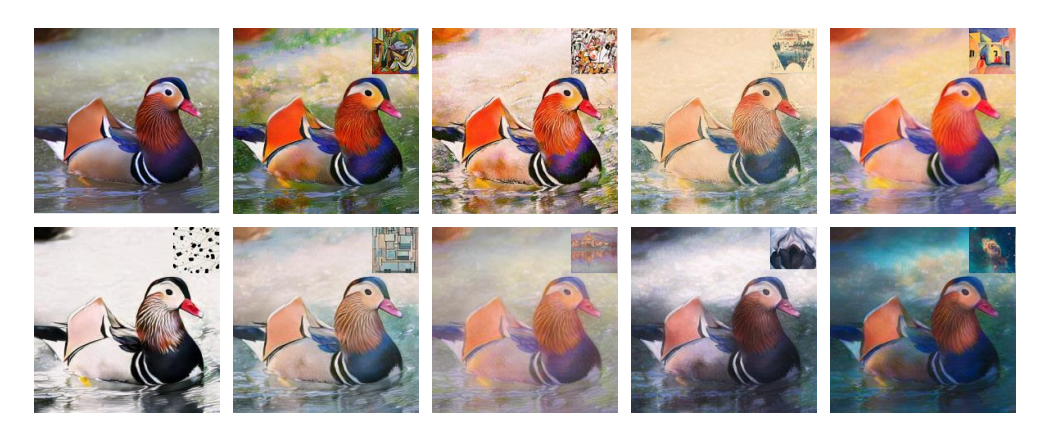
\includegraphics[width=15cm]{teaser.png}
\captionof{figure}{A demo of style tranfer from\cite{ma2023rast}. The top left image is the content image. The style reference image for each synthesized one is shown on the top right corner.
\label{fig:feature-graphic}}
    \label{fig:galaxy}
\end{strip}
%%%%%%%%% ABSTRACT
% \begin{abstract}
%    is to be in fully justified italicized text, at the top of the left-hand column, below the author and affiliation information.
%    Use the word ``Abstract'' as the title, in 12-point Times, boldface type, centered relative to the column, initially capitalized.
%    The abstract is to be in 10-point, single-spaced type.
%    Leave two blank lines after the Abstract, then begin the main text.
%    Look at previous CVPR abstracts to get a feel for style and length.
% \end{abstract}
\section{Motivation}

Neural Style transfer aims to synthesize a new image with its style and content from different reference images. Recently, researchers\cite{gatys2016image} found that certain features in image segmentation neural networks correspond to the style and content semantically. Afterward, many methods\cite{huang2017arbitrary,deng2022stytr2,li2017universal} have been proposed to generate more appealing artistic images in more efficient ways. Our goal is to understand this task through experiments and try to improve on the SOTA methods.

Our work will have two goals in parallel. The first one is to explore extensions and modifications based on existing methods, which could be risky. The second part is to run the code of existing methods on novel data sets, which is more practical. 
In this case, our maximum goal is to design a new method to create artistic images by neural style transfer, which should be comparable to current state-of-the-art methods both qualitatively and quantitatively. Our minimum goal is to use existing methods in a new data set and analyze its performance.
\section{Relationship to Our Background}
Among our four members, Zhengyuan is working on other compute vision topics. He is familiar with deep learning frameworks and general techniques. But he has not done research on this specific topic.
Yifan do not have experience with computer vision regard to image, but he has some other experience like dataset distillation. Yuxuan has not previously participated in computer vision related research. For him, this is an expedition into a new field of computer science. He is familiar with the general principles of software engineering, and will be participating in the research efforts with an engineering perspective. 
Tiansu also has no experience in computer vision, but he worked on several NLP research topics before and is familiar with common deep learning frameworks.
\section{Resources}
We plan to build our code on the publicly available code of a SOTA method\cite{deng2022stytr2}. We will modify different components of their method and try to improve on it. We are also going to adapt their code to novel data sets.

Conceptually, any image set that contains artistic images can be the style dataset.
We plan to use a data set\footnote{https://www.kaggle.com/datasets/thedownhill/art-images-drawings-painting-sculpture-engraving} on Kaggle as our style dataset. For the content dataset, we prefer realistic photos\footnote{https://www.kaggle.com/datasets/tompaulat/modern-architecture-100k-small-images}.
\section{Reservations}
We expect that adapting the code to novel datasets is a problem of time and is mainly dirty work. Also, we could utilize existing code as baselines, which should not be hard. However, since the method itself is powerful, achieving performance improvement could be hard. 

The most difficult part of our project should be the hyperparameter tuning. Neural Style Transfer involves many hyperparameters, such as learning rates, regularization parameters, feature weights. These hyperparameters will impact the quality of the generated images significantly. Also, we need to avoid overfitting, which can result in images that have a distorted or unnatural appearance. Thus, finding the appropriate hyperparameters can be a challenging and time-consuming process, and it may require extensive experimentation and testing.

%%%%%%%%% BODY TEXT
%-------------------------------------------------------------------------
\section{Member roles}
\label{sec:intro}

We divide our project into four parts.

The first one is about research and literature review. Zhengyuan will focus on researching the latest developments in Neural Style Transfer, including any new techniques, architectures, or optimization algorithms that have been proposed in recent literature. 

The second part is data collection and preprocessing: Yifan and Tiansu will focus on collecting and preprocessing the data for the project. This includes finding suitable style and content images, resizing and normalizing the images, and preparing the data for use in the model.

The third part is model development and training: Yifan, Zhengyuan, and Yuxuan will focus on developing and training the Neural Style Transfer model. This involves selecting an appropriate architecture, tuning hyperparameters, and running experiments to find the best model configuration.

Last part is evaluation and analysis: Yuxuan and Tiansu will focus on evaluating the results of the Neural Style Transfer model and conducting a thorough analysis of the model's performance. This includes quantitative analysis of the model's output, as well as qualitative analysis of the artistic quality of the generated images. And all of our four members will write the report when our project is finished. 

All of our four members will schedule regular meetings once a week, to discuss the project's progress and any issues that have come up. What's more, we will set up a shared document, where everyone can contribute their ideas, notes, and updates. All of us can see what's been done and what still needs to be completed on this document. Last, we will use Github to collaborate the coding work. This allows every member to work on their part simultaneously without interfering with each other's work.
%-------------------------------------------------------------------------
\section{Video Style Transfer}

Extending single-frame style transfer to videos requires incorporating the temporal relation between frames to mitigate artifacts. A commonly used prior is optical flow.
The estimation of optical flow is indifferentiable, and thus we can compute the per-pixel loss between the current frame and the wrapped previous frame. We can write the loss as in \cite{huang2017real}:
$$
\textit{L}(\hat{x}^t, \hat{x}^{t-1}) = \frac{1}{D}\sum_{k=1}^D c_k (\hat{x}_k^t-f(\hat{x}_k^{t-1}))^2
$$
where $\hat{x}^t$ and $\hat{x}^{t-1}$ are the stylized frames at adjacant time steps. $f$ is the function that wraps the frame with a pre-computed optical flow. $D$ is the dimension of the output and $c$ is the per-pixel confidence of the optical flow.

Now the problem is how to use this loss. One way\cite{ruder2016artistic} is to directly optimize the generated result, which could lead to slow generation and high quality. Another way\cite{huang2017real,chen2017coherent} is to train a network in order to generate temporally consistent results. We assume that per-frame generation can already give satisfactory results. In this case, we can train an additional RNN to do corrections in order to synthesize temporally coherent videos.

%
%%%%%%%%% REFERENCES
{\small
\bibliographystyle{ieee_fullname}
\bibliography{egbib}
}

\end{document}
